\documentclass[12pt]{article}
\usepackage[utf8]{inputenc}
\usepackage{polski}
\usepackage[a4paper, left=2.0cm, right=2.0cm, top=2.0cm, bottom=2.0cm]{geometry}
\usepackage{hyperref}
\usepackage{graphicx}
\usepackage{listings}

\title{PIISW, W08, IO, 2018/2019, semestr letni\\Lista zadań nr 4}
\author{Michał Luzyna}

\begin{document}
    \maketitle

    \section*{Wprowadzenie}
        Posiadamy system monitorowania zdarzeń na serwerach. Informacje o~zdarzeniach muszą być zapisywane w~relacyjnej bazie danych.

        W~celu realizacji zadania należy zapoznać się z~dokumentacją:
        \begin{itemize}
            \item \href{https://docs.spring.io/spring-data/jpa/docs/current/reference/html/}{Spring data JPA}
            \item \href{https://docs.oracle.com/javaee/6/tutorial/doc/bnbuf.html}{JPQL reference}
        \end{itemize}

        \begin{enumerate}
            \item Utwórz nowe prywatne repozytorium o~nazwie \texttt{imie-nazwisko-lista4} (w~ramach organizacji \texttt{pwr-\allowbreak piisw}) oraz zaimportuj do niego zawartość repozytorium \url{https://github.com/pwr-piisw/jpa-starter}. Projekt zawarty w~repozytorium został zbudowany w~oparciu o~Spring Boot i~wykorzystuje JPA oraz bazę danych H2.
            \item Skonfiguruj \texttt{travis-ci} dla tego repozytorium.
            \item Zapoznaj się ze strukturą klas zaprezentowanych na diagramie z~rysunku~\ref{fig:class-diagram}. Klasy zdarzeń (relacja dziedziczenia) zostały zmapowane z~wykorzystaniem metody \texttt{TABLE\_PER\_CLASS}.
            \item Zapoznaj się z~mapowaniem relacji \texttt{Event} $\rightarrow$ \texttt{Server}.
            \item Baza danych tworzona jest w~momencie startu aplikacji/testów automatycznie dzięki ustawieniu w~pliku \texttt{application.properties}: \texttt{spring\-.jpa\-.hibernate\-.ddl-auto=create}
            \item Zapoznaj się ze skryptem \texttt{data-h2.sql} -- skrypt ten jest uruchamiany przy starcie testów i~ma za zadanie załadowanie danych testowych do bazy.
            \item Zapoznaj się klasami:
                \begin{enumerate}
                    \item \texttt{ServerService} – interfejs usług dotyczących klasy \texttt{Server}
                    \item \texttt{ServerServiceImpl} – implementacja \texttt{ServerService}
                    \item \texttt{ServerRepository} – interfejs DAO dostępu do danych klasy \texttt{Server}. Zauważ, że interfejs ten nie posiada implementacji. Biblioteka \texttt{spring-data} automatycznie generuje kod odpowiedzialny za komunikację z~bazą danych.
                    \item \texttt{ServerServiceTest} – demonstruje działanie klas
                \end{enumerate}
            \item Każde zadanie musi posiadać implementację w~teście o~nazwie \texttt{TaskX} gdzie \texttt{X}~to numer zadania. Dla każdego zadania został przygotowany szablon testu.
        \end{enumerate}
        \begin{figure}[ht]
            \centering
            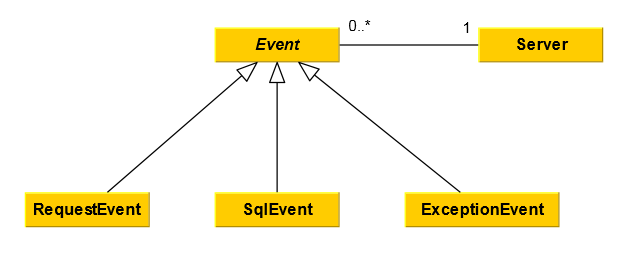
\includegraphics{lista_4_class_diagram}
            \caption{Diagram klas}.
            \label{fig:class-diagram}
        \end{figure}




    \section*{Oceny}
    \begin{tabular}{|l|c|c|c|c|c|c|}
        \hline
        Punkty: & $<9$ & $9-10$ & $11-12$ & $13-14$ & $15-16$ & $17-18$\\
        \hline
        Ocena:  & $2,0$ & $3,0$ & $3,5$ & $4,0$ & $4,5$ & $5,0$\\
        \hline
    \end{tabular}

    \section*{Zadania}
    \begin{enumerate}
        \item
            (2 pkt) Zmodyfikuj klasę Server, dodaj \emph{Optimistic Locking} oraz zaimplementuj aktualizację pola \texttt{lastUpdateDate} o aktualną datę przy każdym zapisie aktualizacji obiektu klasy.

            \textbf{Wskazówka}: wykorzystaj anotacje \texttt{javax.persistence.Version} oraz zaimplementuj \emph{listener} z~wykorzystaniem  adnotacji \texttt{javax.persistence.PreUpdate}.

        \item
            (3 pkt) Utwórz interfejs \texttt{EventRepository} rozszerzający \texttt{org\allowbreak .spring\-frame\-work\allowbreak .data\allowbreak .jpa\allowbreak .re\-po\-si\-to\-ry.Jpa\-Repo\-si\-tory}. Zadeklaruj metodę która dla zadanych parametrów \texttt{Local\-Date\-Time start}, \texttt{Local\-Date\-Time end}, \texttt{boolean toBeAnalyzed} zwróci wszystkie zdarzenia \texttt{Event} które posiadają czas zarejestrowania time taki że \texttt{start} $<$ \texttt{Event.time} $<$ \texttt{end} oraz flaga \texttt{Event.analysisRequired} $=$ \texttt{toBeAnalyzed}.

            \textbf{Wskazówka}: wystarczy nazwać metodę zgodnie z konwencją \texttt{findBy}, \texttt{Between}, \texttt{And}.

        \item
            (2 pkt) Stronicowanie – polega na przekazywaniu danych w porcjach tzw. Stronach. Zadeklaruj w~\texttt{EventRepository} metodę umożliwiającą pobieranie danych z~wykorzystaniem stronicowania.

            \textbf{Wskazówka}: utwórz metodę o nazwie \texttt{findAll}, wykorzystaj \texttt{Page} oraz \texttt{Pageable}.

        \item
            (3 pkt) Usuwanie danych można zrealizować poprzez pobranie obiektów encji oraz wywołanie dla nich metody \texttt{JpaRepository.delete}, istnieje jednak możliwość usuwania danych za pomocą tzw. \emph{Bulk delete}. Zadeklaruj w~\texttt{EventRepository} metodę usuwającą wszystkie zdarzenia \texttt{Event} gdzie \texttt{Event.time} $<$ \texttt{X}. Zadeklaruj \texttt{X} jako \emph{named parameter}.

            \textbf{Wskazówka}: konieczne jest wykorzystanie adnotacji \texttt{@Modifying}, \texttt{@Query}, \texttt{@Param} (z~pakietu \texttt{org\allowbreak .spring\-frame\-work\allowbreak .data})

        \item
            (3pkt) Modyfikację danych można zrealizować poprzez pobranie obiektów encji, a~następnie modyfikacji ich stanu, istnieje jednak możliwość modyfikacji danych za pomocą tzw. \emph{Bulk update}. Zadeklaruj w~\texttt{EventRepository} metodę modyfikującą wszystkie zdarzenia \texttt{Event} określonej podklasy w~ten sposób, że atrybut \texttt{toBeAnalyzed} przyjmie wartość \texttt{'T'}, dla wszystkich zdarzeń spełniających warunek: \texttt{Event.duration} $>$ \texttt{X}. Metoda powinna przyjmować następujące argumenty:
            \begin{itemize}
                \item \texttt{Class<? extends Event> clazz}
                \item \texttt{int minDuration}
            \end{itemize}
            \textbf{Wskazówka}: konieczne jest wykorzystanie adnotacji \texttt{@Modifying}, \texttt{@Query}, \texttt{@Param} (z~pakietu \texttt{org.springframework.data}).

        \item
            (2 pkt) Zadeklaruj w~\texttt{EventRepository} metodę zwracającą listę obiektów typu \texttt{Ser\-ver\-Statis\-tic} --- ile zdarzeń zostało zarejestrowanych na poszczególnych serwerach.

            \textbf{Wskazówka}: konieczne jest wykorzystanie anotacji \texttt{@Query} (z~pakietu \texttt{org\allowbreak .spring\-frame\-work\allowbreak .data}), tzw. JPQL Constructor Expressions oraz klauzuli \texttt{group by}.

        \item
            (3 pkt) Utwórz test zwracający mock zamiast rzeczywistego obiektu. Wykorzystaj w~tym celu \texttt{ServerService.findByName} oraz \texttt{ServerRepository}.

            \textbf{Wskazówka}: zadeklaruj w teście ServerRepository jako  \texttt{@MockBean}, skorzystaj z~\texttt{Mockito\allowbreak .when}, \texttt{Mockito\allowbreak .eq} oraz \texttt{Mockito\allowbreak .thenReturn}.

    \end{enumerate}
\end{document}

